%!TEX TS-program = xelatex
% https://habr.com/ru/post/144648/
\documentclass[a4paper,14pt,ukrainian]{extreport}
\usepackage{xltxtra}

\usepackage{extsizes}
%\usepackage{cmap} % для кодировки шрифтов в pdf
\usepackage{fontspec} 
\defaultfontfeatures{Ligatures={TeX}} 
\setmainfont[Ligatures=TeX]{Times New Roman}
\usepackage[ukrainian]{babel}

\usepackage{graphicx} % для вставки картинок
\usepackage{amssymb,amsfonts,amsmath,amsthm} % математические дополнения от АМС
\usepackage{indentfirst} % отделять первую строку раздела абзацным отступом тоже
\usepackage[usenames,dvipsnames]{color} % названия цветов
\usepackage{makecell}
\usepackage{multirow} % улучшенное форматирование таблиц
\usepackage{ulem} % подчеркивания

\usepackage[nodisplayskipstretch]{setspace}
\onehalfspacing % полуторный интервал
\frenchspacing

\usepackage{fancyhdr}
\pagestyle{fancy}
\fancyhf{}
\fancyhead[R]{\thepage}
\fancyheadoffset{0mm}
\fancyfootoffset{0mm}
\setlength{\headheight}{17pt}
\renewcommand{\headrulewidth}{0pt}
\renewcommand{\footrulewidth}{0pt}
\fancypagestyle{plain}{ 
    \fancyhf{}
    \rhead{\thepage}}
\setcounter{page}{1} 

\usepackage[tableposition=top]{caption}
\usepackage{subcaption}
\DeclareCaptionLabelFormat{gostfigure}{Рис. #2}
\DeclareCaptionLabelFormat{gosttable}{Табл. #2}
\DeclareCaptionLabelSeparator{gost}{~--~}
\captionsetup{labelsep=gost}
\captionsetup[figure]{labelformat=gostfigure}
\captionsetup[table]{labelformat=gosttable}
\renewcommand{\thesubfigure}{\asbuk{subfigure}}

\usepackage{titlesec}
 
\titleformat{\chapter}[display]
    {\filcenter}
    {\bfseries\texorpdfstring{\MakeUppercase{\chaptertitlename}}{{\chaptertitlename}} \thechapter}
    {4pt}
    {\bfseries\MakeUppercase}{}
 
\titleformat{\section}
    {\normalsize\bfseries}
    {\thesection}
    {1em}{}
 
\titleformat{\subsection}
    {\normalsize\bfseries}
    {\thesubsection}
    {1em}{}

% Настройка вертикальных и горизонтальных отступов
\titlespacing*{\chapter}{0pt}{-30pt}{4pt}
\titlespacing*{\section}{\parindent}{*2}{*1}
\titlespacing*{\subsection}{\parindent}{*2}{*1}

\usepackage{geometry}
\geometry{left=3cm}
\geometry{right=1.5cm}
\geometry{top=2.4cm}
\geometry{bottom=2.4cm}

\usepackage{enumitem}
\makeatletter
    \AddEnumerateCounter{\asbuk}{\@asbuk}{м)}
\makeatother
\setlist{nolistsep}
%\renewcommand{\labelitemi}{-}
%\renewcommand{\labelenumi}{\asbuk{enumi})}
%\renewcommand{\labelenumii}{\arabic{enumii})}

\usepackage{tocloft}
\renewcommand{\cfttoctitlefont}{\hspace{0.38\textwidth} \bfseries\texorpdfstring{\MakeUppercase}{}}
\renewcommand{\cftbeforetoctitleskip}{-1em}
%\renewcommand{\cftaftertoctitle}{\mbox{}\hfill \\ \mbox{}\hfill{\footnotesize Стр.}\vspace{-2.5em}}
\renewcommand{\cftchapfont}{\normalsize\bfseries \texorpdfstring{\MakeUppercase{\chaptername}}{{\chaptername}} }
\renewcommand{\cftsecfont}{\hspace{31pt}}
\renewcommand{\cftsubsecfont}{\hspace{11pt}}
\renewcommand{\cftbeforechapskip}{1em}
\renewcommand{\cftparskip}{-1mm}
\renewcommand{\cftdotsep}{1}
\renewcommand{\cftchapleader}{\cftdotfill{\cftdotsep}}
\setcounter{tocdepth}{2} % задать глубину оглавления — до subsection включительно

\newcommand{\empline}{\mbox{}\newline}
\newcommand{\likechapterheading}[1]{ 
    \begin{center}
    \textbf{\texorpdfstring{\MakeUppercase{#1}}{{#1}}}
    \end{center}
    \empline}

\makeatletter
    \renewcommand{\@dotsep}{2}
    \newcommand{\l@likechapter}[2]{{\bfseries\@dottedtocline{0}{0pt}{0pt}{#1}{#2}}}
\makeatother
\newcommand{\likechapter}[1]{    
    \likechapterheading{#1}
    \phantomsection    
    \addcontentsline{toc}{likechapter}{\texorpdfstring{\MakeUppercase{#1}}{{#1}}}}

\usepackage[square,numbers,sort&compress]{natbib}
\renewcommand{\bibnumfmt}[1]{#1.\hfill} % нумерация источников в самом списке — через точку
\renewcommand{\bibsection}{\likechapter{Список літератури}} % заголовок специального раздела
\setlength{\bibsep}{0pt}

\usepackage[title,titletoc]{appendix}
 
\titleformat{\paragraph}[display]
    {\filcenter}
    {\texorpdfstring{\MakeUppercase{\chaptertitlename}}{{\chaptertitlename}} \thechapter}
    {8pt}
    {\bfseries}{}
\titlespacing*{\paragraph}{0pt}{-30pt}{8pt}
 
\newcommand{\append}[1]{  
    \clearpage
    \stepcounter{chapter}    
    \paragraph{\texorpdfstring{\MakeUppercase{#1}}{{#1}}}
    \empline
    \addcontentsline{toc}{likechapter}{
        \texorpdfstring{\MakeUppercase{\chaptertitlename~\Asbuk{chapter}\;#1}}{{\chaptertitlename~\Asbuk{chapter}\;#1}}
    }}

\hyphenation{СУБД}
\usepackage[hidelinks]{hyperref}
\usepackage{microtype}

\begin{document}
\begin{titlepage}
    \thispagestyle{empty}
    \begin{center}
        Міністерство освіти і науки України\\
        Національний технічний університет України\\
        <<Київський політехнічний інститут ім. І. Сікорського>>\\
        Інститут прикладного системного аналізу
    \end{center}
    \vspace{50mm}
    \begin{center}
        \textbf{Курсова робота} \\
        з курсу <<Організація баз даних та знань>> \\
        з теми <<База даних ЗВО>>
    \end{center}
    \vspace{30mm}
    \begin{flushright}
        \textbf{Виконав}: студент 3 курсу \\
        групи КА-81 \\
        Галганов Олексій \\
        \textbf{Прийняла}: асистент \\
        Гуськова Віра Геннадіївна
    \end{flushright}
    \vspace{40mm}
    \begin{center}
        \textbf{Київ 2021}
    \end{center}
\end{titlepage}
\microtypesetup{protrusion=false}
\tableofcontents
\microtypesetup{protrusion=true}
    % !TEX root = ../main.tex
\newpage
\likechapter{Вступ}

ЗВО (заклад вищої освіти) є досить складною системою, в якій непросто описати всі
сутності та зв'язки між ними. Основною задачею бази даних ЗВО є забезпечення зручного
та швидкого доступу до інформації про факультети та кафедри, викладачів та їх навантаження, студентів, розклад.
Необхідно враховувати реальну структуру закладу вищої освіти та зв'язки між наведеними сутностями.

\textbf{Актуальність.} Функціонування такої складної системи, як заклад вищої освіти,
неможливе без використання ефективної інформаційної системи, яка забезпечуватиме 
швидкий та зручний доступ до потрібної інформації.

\textbf{Мета.} Метою роботи є розробка автоматизованої інформаційної системи
для закладу вищої освіти, яка дозволить зберігати всю необхідну інформацію, забезпечить 
виконання всіх видів інформаційних запитів, які необхідні при експлуатації даної 
системи.

\textbf{Завдання.} Спроектувати базу даних та підготувати усі необхідні 
запити та процедури для роботи з нею.

\textbf{Практичне значення.} Вдосконалення навичок SQL-програмування,
аналізу предметної області, проектування баз даних.

\textbf{Програмне забезпечення.} При виконанні роботи було використано
СУБД MySQL 8.0, веб-інтерфейс реалізовано з використанням фреймворку Flask
мови програмування Python 3.9. Використовувалися ОС Windows 10, середовища розробки
Visual Studio Code і MySQL Workbench та система контролю версій Git.
    % !TEX root = ../main.tex
\newpage
\chapter{ПОСТАНОВКА ЗАДАЧІ}
Студенти, організовані в групи, які навчаються на одному з 
факультетів, очолюваному деканатом, в функції якого входить 
контроль навчального процесу. У навчальному процесі беруть 
участь викладачі кафедр, адміністративно відносяться до одного 
з факультетів. Викладачі поділяються на такі категорії: асистенти, 
викладачі, старші викладачі, доценти, професори. Асистенти і 
викладачі можуть навчатися в аспірантурі, ст. викладачі, доценти, 
можуть очолювати наукові теми, професора -- наукові напрямки. 
Викладачі будь-якої категорії свого часу могли захистити 
кандидатську, а доценти і професори і докторську дисертацію, 
при цьому викладачі можуть займати посади доцента і професора 
тільки, якщо вони мають відповідно звання доцента і професора.
Навчальний процес регламентується навчальним планом, в якому 
вказується, які навчальні дисципліни на яких курсах і у яких 
семестрах читаються для студентів кожного року набору, із 
зазначенням кількості годин на кожен вид занять з дисципліни 
(види занять: лекції, семінари, лабораторні роботи, консультації, 
курсові роботи, і т.д.) і форми контролю (залік, іспит). 
Перед початком навчального семестру деканати роздають на кафедри 
навчальні доручення, в яких вказуються будь кафедри (не обов'язково
пов'язані з цим факультетом), які дисципліни і для яких груп
повинні вести в черговому семестрі. Керуючись ними, на кафедрах 
здійснюється розподіл навантаження, при цьому по одній дисципліні 
в одній групі різні види занять можуть вести один або кілька різних
викладачів кафедри (з урахуванням категорії викладачів, наприклад, 
асистент не може читати лекції, а професор ніколи не буде проводити
лабораторні роботи). Викладач може вести заняття по одній або декількох
дисциплінах для студентів як свого, так і інших факультетів. Відомості
про проведені іспитах і заліках збираються деканатом.
Після закінчення навчання студент виконує дипломну роботу, 
керівником якої є викладач кафедри, що відноситься до того 
ж факультету, де навчається студент, при цьому викладач може 
керувати кількома студентами. 

\label{task_list}Види запитів в інформаційний системі:
\begin{enumerate}
    \makeatletter
    \@for\num:={1,2,3,4,5,6,7,8,9,10,11,12,13}\do{
        \item \input{query_descr/\num.txt}
    }
    \makeatother
\end{enumerate}
    % !TEX root = ../main.tex
\newpage
\chapter{Архітектура та інформаційне забезпечення БД}
\section{Аналіз функціонування та організаційні засади підприємства}
До основних функціональних завдань ЗВО належить планування занять та формування їх розкладу,
облік викладачів та студентів, контроль успішності студентів.
Для зберігання необхідних даних доцільно сформувати такі таблиці:
<<Факультети>>, <<Кафедри>>, <<Групи>>, <<Студенти>>, <<Викладачі>>, 
<<Дисципліни>>, <<Розклад>> та <<Сесія>>. На кожному факультеті є кафедри,
за якими закріплені викладачі та навчальні групи студентів. В таблиці <<Дисципліни>>
має бути загальний перелік дисциплін, а вже в таблиці <<Розклад>> -- розподіл
дисциплін за групами та викладачами.

\section{Проектування структури бази даних}
Структуру таблиць БД та зв'язки між ними зображено на EER-діаграмі:
\begin{figure}[h]
    \centering
    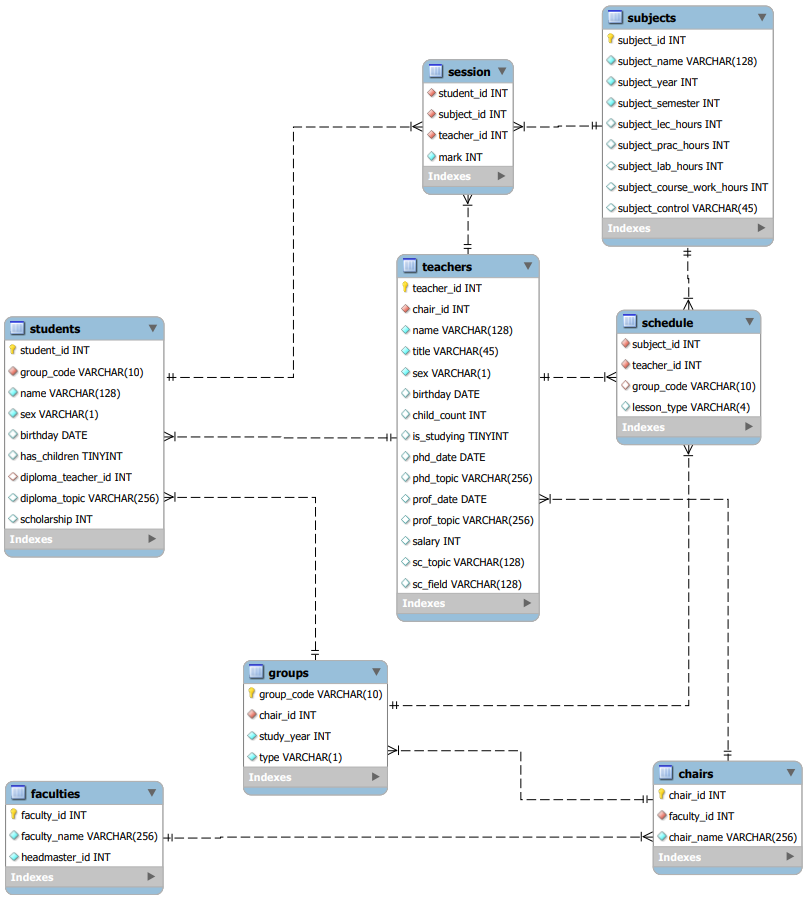
\includegraphics[scale=0.8]{pics/eer.png}
    \caption{EER-діаграма}
\end{figure}

Зв'язки між різними таблицями реалізовано через механізм Foreign Key.
Наприклад, в таблиці <<Сесія>> поля subject\_id, student\_id, teacher\_id 
пов'язані з однойменними полями, що є Primary Key, в таблицях <<Дисципліни>>, <<Студенти>> та <<Викладачі>>.

\section{Життєві цикли бази даних}
\begin{enumerate}
    \item Попереднє планування. На даному етапі було сформовано модель структури бази даних, визначено сутності та
    проаналізовано зв'язки між ними.
    \item Перевірка здійсненності. Для розробки даної системи необхідно мати встановлений сервер MySQL 8.0,
    інтерпретатор мови Python 3.9 з найновішими версіями фреймворку Flask і бібліотеки PyMySQL та
    середовище розробки MySQL Workbench. 
    \item Вимоги до даної інформаційної системи були сформовані в постановці завдання,
    зокрема, вказана структура організації та види інформаційних заходів, які мають бути реалізовані в системі.
    \item Проектування. Для реалізації завдання обрано реляційну модель бази даних. В якості СУБД обрано MySQL.
    Створення початкової структури бази даних (сутності та зв'язки між ними) буде проведено в середовищі MySQL Workbench,
    а реалізацію веб-інтерфейсу доступу до БД та зв'язку між веб-інтерфейсом та MySQL-сервером -- в середовищі Visual Studio Code
    з використанням мови Python та фреймворку Flask.
\end{enumerate}
    % !TEX root = ../main.tex
\newpage
\chapter{Реалізація програмної взаємодії БД}
    % !TEX root = ../main.tex
\newpage

\likechapter{Додатки}

Додаток 1. Створення схеми бази даних.
\lstinputlisting[language=SQL, style=code]{../inserts/create_tables.sql}

\label{setup}Додаток 2. Початкове налаштування бази даних, внесення тестових даних.
\lstinputlisting[language=Python, style=code]{../setup.py}
\end{document}